\documentclass[11pt,a4paper]{article}
\usepackage[utf8]{inputenc}
\usepackage[T1]{fontenc}
\usepackage[margin=0.88in]{geometry}
\usepackage{lmodern}
\usepackage{microtype}
\usepackage{amsmath,amssymb,mathtools}
\usepackage{graphicx}
\usepackage{booktabs,multirow,array}
\usepackage[section]{placeins}
\usepackage[numbers,sort&compress]{natbib}
\usepackage{xcolor}
\usepackage{enumitem}
\usepackage{hyperref}

\hypersetup{
    colorlinks=true,
    linkcolor=blue!50!black,
    citecolor=teal!55!black,
    urlcolor=blue!50!black,
    pdftitle={Uni-3DAR-Mol: Speculative Octree Autoregressive Generation and Sub-Millisecond Seam Healing for Drug-Scale 3D Molecules},
    pdfauthor={Shangqian Chen, Guojiang Zhao, Zheng Cheng, Jiankun Wang, Hongshuai Wang, Zhifeng Gao}
}

\setlength{\emergencystretch}{2em}
\widowpenalty=10000
\clubpenalty=10000
\displaywidowpenalty=10000
\setlength{\parskip}{0.32em}
\setlength{\parindent}{1.2em}
\setlength{\belowcaptionskip}{5pt}
\renewcommand{\topfraction}{0.90}
\renewcommand{\bottomfraction}{0.85}
\renewcommand{\textfraction}{0.08}
\renewcommand{\floatpagefraction}{0.82}

\title{\textbf{Uni-3DAR-Mol: Speculative Octree Autoregressive Generation and Sub-Millisecond Seam Healing for Drug-Scale 3D Molecules}}

\author{
Shangqian Chen, Guojiang Zhao, Zheng Cheng,\\
Jiankun Wang, Hongshuai Wang, Zhifeng Gao\\[4pt]
\small DP Technology, Beijing, China\\
\small\texttt{\{chensq, zhaogj, chengz, wangjk, wanghs, gaozf\}@dp.tech}
}

\date{November 2026}

\begin{document}
\maketitle

\begin{abstract}
Autoregressive generation over adaptive three-dimensional (3D) octrees (\texttt{Uni-3DAR}) offers an intrinsic $\mathcal{O}(N \log N)$ spatial sparsity advantage over dense $\mathcal{O}(N^2)$ multi-step equivariant diffusion and flow-matching models on large drug-like molecules. Yet in practice, unbonded octree autoregressive models have lagged behind joint 2D+3D flow-matching architectures in geometric equilibrium quality, closed-shell valence stability, and size-controlled conditional generation due to three structural pathologies: (i) \emph{Morton-order voxel-seam coordinate discontinuities} that induce severe zero-step interatomic force spikes ($F_{\max} \approx 3.8\text{--}5.0\,\text{eV/\AA}$) and $15\%\text{--}26\%$ exotic zwitterionic bond-perception artifacts when covalent bonds cross octant boundaries; (ii) \emph{unpruned leaf compute dominance and root-count trapping}, where fine leaf-atom and $0.01\,\text{\AA}$ coordinate tokens consume over $70\%$ of decoding latency even on dead-end coarse scaffolds while hard octant count splits starve large scaffolds ($N \ge 45$); and (iii) \emph{cross-scale gradient interference} between coarse spatial/chemical tokens and $3\times$ more numerous sub-voxel coordinate bins during post-training alignment. Here we introduce \textbf{Uni-3DAR-Mol}, a next-generation 3D octree autoregressive architecture and speculative tree-decoding engine that resolves all three bottlenecks with zero inference-time machine-learning interatomic potential (MLIP) relaxation. \textbf{Uni-3DAR-Mol} combines: (1) non-trapping 6-D scale-free atom-budget modulation paired with hierarchical covalent packing priors ($\text{L5}\to\text{L1}$); (2) a vectorized FlashAttention2 pause-and-gather \emph{speculative octree funnel} $m_{\text{s1}}(M,\hat{N}) \to m_{\text{s2}}(M,\hat{N}) \to M$ governed by a continuous combinatorial complexity law and a $3$-layer $\text{SO}(3)$-invariant GNN \texttt{TwoStageOctreeProcessCritic} trained with group-wise ListNet, pairwise ranking, and physical strain ($F_{\text{phys}}$) objectives; (3) a $<0.5\,\text{ms}$ $4$-layer Kabsch-aligned $SE(3)$ \texttt{PostTreeGraphRefiner} with a bilinear covalent bond-order head coupled to generation-side neutral valence guards and a zero-heavy-displacement \texttt{ValenceReconciler}; (4) scale-decoupled \texttt{Tree-Vine TopoGRPO} plus differentiable expected-\texttt{XYZ} 1--2/1--3 bonded-distance supervision; and (5) bubble-free stride-2 GPU leaf decoding. Across unconditional drug-scale generation on \texttt{GEOM-Drugs} ($10{,}000$ molecules, $14$ elements, up to $140$ atoms; $0.49\,\text{GPU-h}$ post-training), asymptotic scaling up to $N=100$ explicit atoms, six-property conditional generation on the disjoint $50\text{k}/50\text{k}$ \texttt{QM9} benchmark ($1 \times K=6$ unified model, $0.66\,\text{GPU-h}$), and symmetric multi-tier ($M \in \{1,2,4,8,12,16\}$) optoelectronic inverse design on \texttt{OE62} verified by live \texttt{GPU4PySCF PBE0/def2-TZVP} quantum chemistry ($2.41\,\text{GPU-h}$), \textbf{Uni-3DAR-Mol} lifts drug-scale valid-connected yield $6.78\times$ ($12.7\% \to 86.2\%$, $99.83\%$ explicit atom stability), runs up to $7.3\times$ faster ($M=1$) or $1.65\times$ faster with $2.0\times$ higher valid-connected yield ($M=2$) than dense $100$-step \texttt{FlowMol} at $N=100$, beats $6$-model \texttt{PropMolFlow} ($156\,\text{GPU-h}$) on intensive \texttt{QM9} targets ($\mu, \varepsilon_{\text{HOMO}}, \Delta\varepsilon$), and surpasses $52.12\,\text{GPU-h}$ aligned flow matching on \texttt{OE62} by $+40\%$ in 3D quality index ($Q_{\text{3D}}$), $+7.1\,\text{pp}$ in $M=8$ blind hit yield, sub-$2\,\text{eV/\AA}$ zero-step force equilibrium, and $64.3\%\text{--}69.0\%$ live \texttt{PBE0} quantum hit yield at $21.6\times$ lower training compute.
\end{abstract}

\section{Introduction}
\label{sec:intro}

De novo generation of three-dimensional (3D) molecular structures lies at the core of structure-based drug discovery \citep{axelrod2022geom,dunn2024flowmol,irwin2025semlaflow} and functional optoelectronic materials design \citep{stuke2020oe62,zeng2026propmolflow}. Dominant 3D molecular generative paradigms currently fall into two families with sharply contrasting computational and physical trade-offs:

\begin{enumerate}[leftmargin=1.6em,itemsep=2pt,topsep=3pt]
    \item \textbf{Dense Iterative Equivariant Diffusion and Flow Matching.} Early coordinate-only diffusion models (\texttt{EDM} \citep{hoogeboom2022edm}, \texttt{GeoLDM} \citep{xu2023geoldm}) require $500\text{--}1{,}000$ $E(3)$-equivariant message-passing steps over complete graphs and suffer catastrophic molecule-level valence instability on drug-sized molecules ($0.2\%\text{--}5.2\%$ on \texttt{GEOM-Drugs}). Joint 2D+3D diffusion and continuous-time Markov chain (CTMC) flow-matching models (\texttt{MiDi} \citep{vignac2023midi}, \texttt{EQGAT-diff} \citep{le2023eqgatdiff}, \texttt{FlowMol} \citep{dunn2024flowmol}, \texttt{SemlaFlow} \citep{irwin2025semlaflow}, \texttt{PropMolFlow} \citep{zeng2026propmolflow}) explicitly co-evolve all $N(N-1)/2$ pairwise bond states alongside 3D coordinates over $100\text{--}500$ ODE/SDE steps. While explicit edge evolution restores chemical validity, materializing dense $\mathcal{O}(N^2)$ pair representations at every integration step incurs steep wall-clock latency and memory scaling as $N$ grows from $30$ to $100$ explicit atoms, and lacks exact trajectory log-likelihoods for sample-efficient reinforcement learning (RL).
    \item \textbf{Sparse Hierarchical 3D Octree Autoregression.} \texttt{Uni-3DAR} \citep{lu2025uni3dar} recursively partitions 3D space from a coarse cubic root ($L=6$ or $7$, box side $15.36\text{--}30.72\,\text{\AA}$) down to $0.24\,\text{\AA}$ leaf cells ($L=0$) in breadth-first Morton ($Z$-curve) order, emitting only non-empty spatial octants ($\mathcal{O}(N \log N)$ tokens) followed by chemical element identity $Z_i$ and quantized $0.01\,\text{\AA}$ sub-voxel offsets $(\Delta x_i, \Delta y_i, \Delta z_i)$. This formulation provides exact autoregressive log-probabilities and single-pass causal KV-cached decoding.
\end{enumerate}

Despite its compelling $\mathcal{O}(N \log N)$ asymptotic complexity, deploying vanilla octree autoregression on drug-scale benchmarks (\texttt{GEOM-Drugs}, $N \approx 47$ mean atoms, up to $140+$ atoms) and stringent multi-constraint conditional tasks (\texttt{OE62}) exposes three fundamental failure modes that have prevented octree models from overtaking explicit-bond flow matching:

\begin{itemize}[leftmargin=1.5em,itemsep=2pt,topsep=3pt]
    \item \textbf{Pathology 1: Morton-Seam Force Spikes and Unbonded Zwitterionic Fragility.} When two covalently bonded atoms fall on opposite sides of a coarse octree division plane, their sub-voxel coordinates are decoded far apart in the causal sequence without explicit pairwise bond springs. Small $0.03\text{--}0.08\,\text{\AA}$ cross-seam misalignments produce severe zero-step interatomic force spikes (median $F_{\max} \approx 3.9\,\text{eV/\AA}$, $90$th percentile $>17\,\text{eV/\AA}$ under \texttt{DPA-4} \citep{deepmodeling2026dpa4}). Simultaneously, omitting or misplacing a single $0.31\,\text{\AA}$ peripheral hydrogen forces post-hoc distance-based bond perception (\texttt{RDKit DetermineBonds} \citep{rdkit2026bonds}) to invent high-energy zwitterions (\texttt{[C-]...[O+]}, trivalent oxonium, halonium) on $15\%\text{--}26\%$ of structures.
    \item \textbf{Pathology 2: Leaf-Heavy Compute Allocation and Coarse Count Trapping.} In an octree sequence, coarse spatial tree splits ($L \ge 1$) occupy fewer than $30\%$ of total compute, whereas fine leaf-atom and $3$-axis $0.01\,\text{\AA}$ coordinate heads consume $>70\%$. Naive best-of-$M$ sampling wastes full leaf rollout compute on topologically strained or off-target coarse envelopes. Moreover, conditioning octant subdivisions on rigid remaining-atom counters traps large molecules ($N \ge 45$) when early coarse octants under-allocate sub-volumes.
    \item \textbf{Pathology 3: Cross-Scale Policy-Gradient Interference and Host-Device Sync Bubbles.} Propagating scalar molecular rewards equally through coarse topology tokens and $3\times$ more numerous $0.01\,\text{\AA}$ coordinate tokens degrades conditional property precision, while standard dynamic queue decoding triggers $>200$ GPU--CPU synchronization stalls (\texttt{.item()}, \texttt{nonzero()}) per batch.
\end{itemize}

In this paper, we present \textbf{Uni-3DAR-Mol}, a principled architectural and inference-engine redesign of 3D octree autoregressive molecular generation. Strictly adhering to zero PCA canonicalization (full $\text{SO}(3)$ equivariant augmentation) and zero inference-time MLIP relaxation, \textbf{Uni-3DAR-Mol} introduces five synergistic innovations:
\begin{enumerate}[leftmargin=1.6em,itemsep=1pt,topsep=2pt]
    \item \textbf{Scale-Free Non-Trapping Budget Modulation \& Hierarchical Packing Priors (Section~\ref{sec:budget}):} A zero-initialized 6-D continuous global scale embedding paired with empirical $\text{L5}\to\text{L1}$ organic packing priors that smoothly expand $N=20\text{--}100+$ scaffolds without conditioner leakage or octant count trapping;
    \item \textbf{Speculative Two-Stage Octree Tree Decoding \& Combinatorial Scaling Law (Section~\ref{sec:spectree}):} A FlashAttention2 pause-and-gather KV funnel $m_{\text{s1}}(M,\hat{N}) \to m_{\text{s2}}(M,\hat{N}) \to M$ pruned at $L=1\to 0$ and $L=0$ by a $3$-layer $\text{SO}(3)$-invariant GNN \texttt{TwoStage\allowbreak Octree\allowbreak ProcessCritic} trained with group-wise ListNet, pairwise logistic, and zero-step $F_{\text{phys}}$ ranking losses;
    \item \textbf{Sub-Millisecond Kabsch \texttt{PostTreeGraphRefiner} \& Dual-Track Valence Engine (Section~\ref{sec:refiner}):} A $<0.5\,\text{ms}$ $4$-layer $SE(3)$-equivariant coordinate refiner and bilinear bond-order head distilled on equilibrium conformers, coupled with pre-softmax neutral coordination guards (\texttt{HeavyAtomValenceHead}) and a zero-heavy-displacement \texttt{ValenceReconciler};
    \item \textbf{Scale-Decoupled \texttt{Tree-Vine TopoGRPO} \& Differentiable Expected-\texttt{XYZ} Supervision (Section~\ref{sec:alignment}):} Separating coarse-topology RL from expected-$0.01\,\text{\AA}$ 1--2/1--3 bonded distance supervision and detached sub-voxel equilibrium distillation;
    \item \textbf{Bubble-Free Stride-2 GPU Decoding \& Dynamic VRAM Scheduling (Section~\ref{sec:engine}):} Eliminating $>95\%$ of host-device synchronization stalls while scaling Stage-1 KV capacity dynamically with live GPU memory and target atom budget.
\end{enumerate}

\section{The Uni-3DAR-Mol Architecture and Decoding Engine}
\label{sec:method}

\subsection{Scale-Free Global Budget Modulation and Hierarchical Volume Conservation}
\label{sec:budget}

Let an octree of root merge level $L_{\max} \in \{6, 7\}$ ($0.24\,\text{\AA}$ leaf voxel width) represent a 3D molecule $\mathcal{M} = \{(Z_i, \mathbf{r}_i)\}_{i=1}^N$. In standard \texttt{Uni-3DAR}, autoregressive root-count prediction commits early coarse octants to integer atom quotas $c_{\text{alloc}}$, causing steric overcrowding on small molecules or premature termination on $N \ge 50$ drug scaffolds. Crucially, injecting $N$ into a property conditioner conflates intrinsic intensive electronic properties (e.g., frontier orbital energies) with extensive molecular size.

\textbf{Uni-3DAR-Mol} decouples extensive size control entirely from property conditioning via two mechanisms:
\begin{enumerate}[leftmargin=1.6em,itemsep=2pt,topsep=2pt]
    \item \textbf{Non-Trapping 6-D \texttt{ScaleFreeBudgetEmbedding}:} Every non-EOT octree token at level $\ell \in \{0, \dots, L_{\max}\}$ receives a zero-initialized residual embedding $\phi_{\text{budget}}(\ell, N) \in \mathbb{R}^d$ computed purely from dimensionless log-scale and harmonic features of total target atom budget $N$:
    \begin{equation}
    \label{eq:budget_emb}
    \begin{aligned}
    \mathbf{z}_{\text{budget}}(\ell, N) = \Big[&\mathbb{I}_{N>0},\; \frac{\log(1+N)}{4.5},\; \operatorname{clip}\!\left(\frac{N-30}{25}, -2.5, 4.5\right), \\
    &\frac{\ell+1}{8},\; \sin\!\left(\pi \log\frac{N}{30}\right),\; \cos\!\left(\pi \log\frac{N}{30}\right)\Big],
    \end{aligned}
    \end{equation}
    trained with $p_{\text{drop}} = 0.12$ budget dropout so a single checkpoint seamlessly supports both exact-budget and unbudgeted free generation across $N \in [16, 140]$ without per-octant integer trapping.
    \item \textbf{Physics-Informed Hierarchical Packing Priors ($\text{L5}\to\text{L1}$):} During coarse tree expansion ($1 \le \ell \le 5$), let $R_\ell$ denote the number of remaining unexpanded cells at level $\ell$ and $C_{\ell-1}$ the child cells already spawned at level $\ell-1$. Empirical equilibrium organic conformers obey tight characteristic occupancy ratios $N / N_{\text{cells}}(\ell) \approx (3.00, 1.36, 0.99, 0.99, 0.99)$ from $\ell=5$ ($7.68\,\text{\AA}$) down to $\ell=1$ ($0.48\,\text{\AA}$). For any 8-bit non-empty split mask $u \in \{1,\dots,255\}$ with popcount $k(u) = \|u\|_1$, we shift only the cardinality prior while preserving all $\binom{8}{k}$ spatial octant orientations:
    \begin{equation}
    \label{eq:vol_prior}
    \tilde{\ell}_{\text{tree}}(u) = \ell_{\text{tree}}(u) - w_\ell \left(k(u) - \operatorname{clip}\!\left(\frac{N/\delta_\ell - C_{\ell-1}}{R_\ell},\, 1,\, \kappa_\ell\right)\right)^2 + \mathcal{P}_{\text{steric}}(u; \ell),
    \end{equation}
    where coarse envelopes ($\ell \in \{3,4,5\}$) apply gentle soft quadratic guidance ($w_\ell \propto g_{\text{scale}}$) to prevent fragmentation on $N=50\text{--}100$ molecules while fine $0.96/0.48\,\text{\AA}$ cells ($\ell \in \{1,2\}$) enforce strict steric leaf caps ($k(u) \le 2$) to prevent atomic collisions.
\end{enumerate}

\subsection{Speculative Two-Stage Octree Decoding and Combinatorial Complexity Law}
\label{sec:spectree}

\paragraph{Continuous Combinatorial Tree-Branching Law.}
Given an external candidate budget $M \in \{1, 2, 4, 8, 12, 16\}$ (standardized service tiers \texttt{base/low/medium/high} plus extended \texttt{ext/xhigh}), decoding all $M$ trajectories from root to $0.01\,\text{\AA}$ leaves under-utilizes the fast coarse octree prefix ($\ell \ge 1$). Conversely, fixing a static coarse fan-out (such as $64 \to 16 \to 8$) wastes compute on small rigid scaffolds ($N \le 20$) where a $9\text{--}14$ heavy-atom space saturates quickly, while larger flexible scaffolds ($N \ge 30$) require wide prefix exploration to avoid strained ring closures. We introduce a smooth combinatorial complexity factor $\eta(\hat{N}) = \operatorname{clip}((\hat{N} - 16)/14,\, 0,\, 1)$ ($\eta = 1$ when unbudgeted) over median batch atom budget $\hat{N}$, defining even-integer internal widths while strictly locking outer output count at $m_{\text{keep}} \equiv M$:
\begin{equation}
\label{eq:funnel_law}
m_{\text{s1}}(M, \hat{N}) = 2 \left\lceil \frac{M \big(4 + 4\,\eta(\hat{N})\big)}{2} \right\rceil, \qquad
m_{\text{s2}}(M, \hat{N}) = 2 \left\lceil \frac{M \big(1.25 + 0.75\,\eta(\hat{N})\big)}{2} \right\rceil, \qquad (M > 1),
\end{equation}
and $(1 \to 1 \to 1)$ for $M=1$. Thus Eq.~\eqref{eq:funnel_law} adapts seamlessly from compact \texttt{QM9} prompts ($\hat{N} \approx 18$: $10\to 4\to 2$, $20\to 6\to 4$, $38\to 12\to 8$, $74\to 22\to 16$) through $N=20$ ($42\to 12\to 8$ at $M=8$) to full drug/optoelectronic scaffolds ($\hat{N} \ge 30$: $16\to 4\to 2$, $32\to 8\to 4$, $64\to 16\to 8$, $96\to 24\to 12$, $128\to 32\to 16$).

\paragraph{Vectorized Pause-and-Gather Funnel and Ranking \texttt{TwoStageOctreeProcessCritic}.}
For a batch of $B_p$ prompts, \textbf{Uni-3DAR-Mol} executes two internal GPU pruning stages without external oracle or MLIP calls:
\begin{enumerate}[leftmargin=1.6em,itemsep=2pt,topsep=2pt]
    \item \textbf{Stage 1 (Coarse Envelope Pruning, $B_p m_{\text{s1}} \to B_p m_{\text{s2}}$):} All $B_1 = B_p m_{\text{s1}}$ trajectories decode coarse octree splits ($\ell \ge 1$) in parallel and pause in-place immediately upon reaching their first $\ell = 0$ leaf token. \texttt{OctreeProcessCritic} fuses pooled root/coarse/$\text{L1}$ Transformer hidden states ($4d$) with $14$ exact $\text{SO}(3)$-invariant voxel-envelope descriptors (leaf count $K_0$, radius of gyration $R_g$, principal inertia eigenvalues $\lambda_{1\ge 2\ge 3}$, anisotropy/planarity ratios, nearest-neighbor packing, and coarse perplexity) to retain the top-$m_{\text{s2}}$ coarse prefixes per prompt, gathering only winning KV-cache rows via a single vectorized \texttt{index\_select} per layer and freeing $75\%\text{--}80\%$ of KV memory before leaf decoding.
    \item \textbf{Stage 2 (3D Element-Cloud GNN Pruning \& MMR Diversity, $B_p m_{\text{s2}} \to B_p M$):} Surviving prefixes decode $\ell = 0$ leaf atoms and coordinates. \texttt{Octree\allowbreak Element\allowbreak ProcessCritic} runs a $3$-layer $\text{SO}(3)$-invariant radial-basis message-passing GNN ($24$ Gaussian RBFs over $d_{ij} \in [0.5, 5.0]\,\text{\AA}$) over placed 3D atoms fused with $36$ stoichiometric and pairwise clash/coordination features, selecting the final $M$ candidates via greedy Maximal Marginal Relevance (MMR) hinge deduplication ($\operatorname{sim} > 0.93$) to prevent sibling-leaf collapse from identical coarse trunks.
\end{enumerate}
Both critic stages are trained jointly on grouped on-policy rollouts ($G=8$) with composite regression, within-group ListNet KL, pairwise logistic ranking, and offline post-refiner \texttt{DPA-4} physical equilibrium score $R_{\text{phys}}(F_{\text{rms}}, F_{\max}) = \exp(-\max(0, F_{\max} - 0.40)/2.0)$, teaching the internal GNN to prune strained or valence-defective prefixes before bond perception.

\subsection{Sub-Millisecond Kabsch Seam Healing and Dual-Track Valence Purity}
\label{sec:refiner}

\paragraph{$SE(3)$-Equivariant \texttt{PostTreeGraphRefiner}.}
To eliminate Morton octant-seam coordinate jumps without iterative inference-time force-field relaxation, we design a lightweight $4$-layer $SE(3)$-equivariant graph transformer ($d_{\text{model}} = 192$, $4$ heads, $24$ distance RBFs, $<0.5\,\text{ms}$ per batched call) applied once to raw decoded leaf clouds $\{(\hat{Z}_i, \hat{\mathbf{r}}_i)\}_{i=1}^N$. Each layer updates scalar node embeddings $\mathbf{h}_i^{(\ell)}$, pairwise edge states $\mathbf{e}_{ij}^{(\ell)}$ ($d_{ij} < 3.4\,\text{\AA}$), and bounded zero-CoM equivariant coordinate displacements:
\begin{equation}
\label{eq:refiner}
\Delta \mathbf{r}_i^{(\ell)} = \frac{1}{\mathcal{N}_i} \sum_{j \in \mathcal{N}(i)} \psi_x\!\left(\mathbf{e}_{ij}^{(\ell)}\right) \frac{\mathbf{r}_i^{(\ell)} - \mathbf{r}_j^{(\ell)}}{\|\mathbf{r}_i^{(\ell)} - \mathbf{r}_j^{(\ell)}\| + \epsilon}, \qquad
\mathbf{r}_i^{\text{out}} = \hat{\mathbf{r}}_i + 0.25 \tanh\!\left(\frac{\tilde{\mathbf{r}}_i - \hat{\mathbf{r}}_i}{0.25}\right),
\end{equation}
accompanied by a symmetric bilinear head predicting continuous covalent bond-order probabilities $P(b_{ij} \in \{0, 1, 2, 3, \text{arom}\})$. Crucially, we train \texttt{PostTreeGraphRefiner} on equilibrium conformers augmented with synthetic random-$\text{SO}(3)$ octant-plane Morton shifts \emph{plus} real on-policy rollouts relaxed offline by \texttt{DPA-4} and superimposed via exact Kabsch alignment ($\det \mathbf{R} = +1$), supervising 1--2/1--3 pairwise distances, Kabsch Huber coordinate error, and cross-entropy bond orders.

\paragraph{Dual-Track Zero-Heavy-Displacement Valence Engine.}
In parallel, \textbf{Uni-3DAR-Mol} eliminates unbonded zwitterionic bond-perception failures via: (i) \textbf{Track A (Decoding-Time Coordination Guard + \texttt{HeavyAtomValenceHead}):} pre-softmax masking of covalent bonding logits near saturated oxygen ($\text{C=O}$ at $d<1.28\,\text{\AA}$ or $2$ single neighbors), monovalent halogens ($\text{F, Cl, Br, I}$), and trivalent neutral boron, backed by an SFT auxiliary valence head; and (ii) \textbf{Track B (\texttt{ValenceReconciler}):} returning already-clean point clouds untouched while repairing isolated peripheral-H mismatches on intact single-component heavy skeletons at exact $\text{RMSD}_{\text{heavy}} \equiv 0.0000\,\text{\AA}$ using \texttt{PostTreeGraphRefiner}'s bilinear bond-order priors (\texttt{potential\_slot=None}, zero inference MLIP calls).

\subsection{Scale-Decoupled Alignment and Differentiable Sub-Voxel Geometry}
\label{sec:alignment}

During supervised adaptation, we augment discrete $0.01\,\text{\AA}$ \texttt{XYZ}-bin cross-entropy with a training-only differentiable expected-coordinate geometric loss over softmax-expected sub-voxel positions $\bar{\mathbf{r}}_i = \mathbf{o}_i + \delta_{xyz} \sum_b b \, p_i(b)$, supervising 1--2 covalent bonds ($d_{ij}^{\text{gt}} < 1.85\,\text{\AA}$, weight $2.0$) and 1--3 geminal bond angles ($d_{ij}^{\text{gt}} < 2.65\,\text{\AA}$, weight $1.0$) via Smooth-$L_1$ loss at $0\%$ inference overhead. For conditional tasks (\texttt{OE62}), we decouple coarse-topology group-relative policy optimization (\texttt{Tree-Vine TopoGRPO} over $\mathcal{T}_{\text{topo}}$ with exact dual-finite token KL and tree-depth-annealed selective logit-CFG: $s_{\text{CFG}}$ on tree/element heads, $1.0$ on \texttt{XYZ} heads) from detached rank-$8$ \texttt{XYZ}-head equilibrium coordinate distillation (\texttt{hidden.detach()}).

\subsection{Bubble-Free GPU Decoding and Dynamic VRAM Scheduling}
\label{sec:engine}

Standard Python-driven octree queues incur $>10$ CUDA host-device synchronizations per step via boolean indexing and \texttt{.item()} emptiness checks. \textbf{Uni-3DAR-Mol} introduces: (i) \texttt{gather/scatter\_} masked buffer writes and \texttt{scatter\_add\_} cell-counter updates in Stage~1, keeping \texttt{prebuilt\_attn\_mask=None} (native FlashAttention2) across all pre-pause coarse steps and polling completion only every $4$ steps; (ii) direct stride-$2$ placed-atom slicing (\texttt{dec\_feat[:, max\_dec\_0+1 : dec\_len : 2]}) in Stage~2, eliminating full-sequence scans and boolean column gathers while compacting finished leaf rows every $6$ steps; and (iii) tight budget-proportional KV allocation ($T_{\max} = \max(96, 3\lceil N_{\max}\rceil + 48 + 8(L_{\max}-6))$, with Stage-1 KV capped to coarse depth $\approx 1.9 N_{\max} + 36$) paired with live \texttt{cuda.mem\_get\_info} chunk sizing and automatic OOM half-batch retry.

\section{Experiments}
\label{sec:experiments}

We evaluate \textbf{Uni-3DAR-Mol} across three complementary benchmarks under strict zero-PCA ($\text{SO}(3)$ random rotation $p=0.80$), zero-$N_{\text{atoms}}$ property-conditioner leakage, and zero-inference-MLIP protocols on single NVIDIA A800-SXM4-80GB GPUs: (1) $10{,}000$-molecule unconditional drug-scale 3D generation and $N \in \{30, 45, 60, 80, 100\}$ asymptotic scaling on \textbf{\texttt{GEOM-Drugs}} \citep{axelrod2022geom} ($L_{\max}=7$, $14$ main-group elements $\text{H, B, C, N, O, F, Si, P, S, Cl, As, Se, Br, I}$); (2) six-property conditional generation on the leakage-free $50\text{k}/50\text{k}$ disjoint \textbf{\texttt{QM9}} benchmark \citep{ramakrishnan2014qm9,zeng2026propmolflow} ($L_{\max}=6$, $N=1{,}000$ held-out prompts per property, $0$ overlap with \texttt{gvp\_rQM\_v0}); and (3) symmetric multi-tier ($M \in \{1, 2, 4, 8, 12, 16\}$) optoelectronic inverse design, $2 \times 2$ mechanism ablations, and $N \in \{20, 30, 40, 50, 60\}$ controlled size scaling on \textbf{\texttt{OE62}} \citep{stuke2020oe62} verified by live \texttt{GPU4PySCF PBE0/def2-TZVP/DF} \citep{sun2020pyscf,li2024gpu4pyscf}.

\subsection{Drug-Scale Unconditional Generation and $N=30\text{--}100$ Scaling on GEOM-Drugs}
\label{sec:exp_geom}

Starting from the public unconditional \texttt{Uni-3DAR} (\texttt{drug.pt}) checkpoint, \textbf{Uni-3DAR-Mol} requires only $\mathbf{0.4914\,\text{GPU-h}}$ of total post-training on \texttt{GEOM-Drugs}: $0.1479\,\text{GPU-h}$ of full-$\text{SO}(3)$ supervised adaptation with \texttt{ScaleFreeBudgetEmbedding} and differentiable expected-\texttt{XYZ} 1--2/1--3 bonded-distance loss, $0.0587\,\text{GPU-h}$ ($12$ epochs) of \texttt{PostTreeGraphRefiner} distillation (reducing validation noisy bond-length MAE from $0.0668\,\text{\AA}$ to $\mathbf{0.0126\,\text{\AA}}$ at $\mathbf{99.27\%}$ bond-order classification accuracy), and $0.2848\,\text{GPU-h}$ of grouped rollout fitting for \texttt{TwoStageOctreeProcessCritic} ($99.26\%\text{--}99.39\%$ constraint-head accuracy).

Table~\ref{tab:geom}a and Figure~\ref{fig:geom}a,c compare \textbf{Uni-3DAR-Mol} against pretrained \texttt{Vanilla Uni-3DAR} and published coordinate-only diffusion (\texttt{EDM}, \texttt{GeoLDM}) as well as explicit-edge joint 2D+3D diffusion/flow-matching baselines (\texttt{MiDi-Adaptive}, \texttt{EQGAT-diff}, \texttt{FlowMol}, \texttt{SemlaFlow}) across $10{,}000$ sampled drug-scale conformers ($100.0\%$ uniqueness and $100.0\%$ novelty across all octree arms). Because \texttt{Vanilla Uni-3DAR} suffers cross-octant Morton-seam jumps and unguarded peripheral-H omissions, raw distance-based bond perception yields only $19.60\%$ validity, $12.70\%$ valid-and-connected molecules, and $6.42\%$ explicit molecule stability ($8.03\,\text{eV/\AA}$ median $F_{\max}$). Even at single-pass $M=1$ ($25.88\,\text{mol/s}$, $38.65\,\text{s/1k}$), \textbf{Uni-3DAR-Mol} lifts valid-and-connected yield $4.05\times$ to $51.41\%$ ($99.69\%$ explicit atom stability, $45.14\%$ molecule stability). Activating the speculative octree funnel at $M=2$ ($16\to 4\to 2$, $7.67\,\text{mol/s}$, $|\Delta N|=2.31$) and $M=4$ ($32\to 8\to 4$, $4.00\,\text{mol/s}$, $|\Delta N|=2.35$) drives \texttt{Valid \& Connected} up $\mathbf{6.78\times}$ to $\mathbf{86.15\%}$---surpassing $500$-step explicit-edge \texttt{MiDi-Adaptive} ($77.8\%$) without evolving dense $\mathcal{O}(N^2)$ bond matrices---while matching joint flow-matching atom-level valence stability ($\mathbf{99.83\%}$ vs.\ $99.7\%\text{--}99.8\%$) and lifting explicit molecule stability $\mathbf{12.5\times}$ to $\mathbf{80.15\%}$ ($15.4\times$ higher than coordinate-only \texttt{GeoLDM} at $5.2\%$). Simultaneously, 3D geometric distributions tighten sharply against held-out \texttt{GEOM-Drugs} conformers (Figure~\ref{fig:geom}c): mean bond-length Jensen--Shannon divergence (JSD) drops to $0.0951$ (aromatic $\text{C=C}$ JSD $0.0730 \to \mathbf{0.0207}$ at $1.392\,\text{\AA}$; aromatic $\text{C=N}$ JSD $0.0507 \to \mathbf{0.0152}$ at $1.345\,\text{\AA}$; $\text{C--H}$ $1.093\,\text{\AA}$), bond-angle JSD drops $-36.6\%$ ($0.0516 \to 0.0327$), ring-size JSD drops $-47.8\%$ ($0.0471 \to 0.0246$), strained 3/4-membered ring fraction drops $-49.4\%$ ($12.35\% \to 6.25\%$), and $90$th-percentile zero-step \texttt{DPA-4} force falls from $17.34$ to $13.92\,\text{eV/\AA}$.

To directly test $\mathcal{O}(N \log N)$ octree sparsity against $\mathcal{O}(N^2)$ pair-matrix flow matching on identical A800 hardware, Table~\ref{tab:geom}b and Figure~\ref{fig:geom}b evaluate exact target sizes $N \in \{30, 45, 60, 80, 100\}$ ($250$ molecules/bucket) head-to-head against $100$-step \texttt{FlowMol}. As $N$ grows from $30$ to $100$ explicit atoms, dense pair-feature updates slow \texttt{FlowMol} $8.6\times$ ($53.8 \to 463.1\,\text{s/1k}$, $2.16\,\text{mol/s}$) while its valid-connected yield collapses from $97.6\%$ to $14.0\%$ ($0.4038$ bond JSD, $28.5\%$ strained small rings). In contrast, \textbf{Uni-3DAR-Mol} ($M=1$) scales gently from $18.7$ to $\mathbf{63.4\,\text{s/1k}}$ ($\mathbf{15.79\,\text{mol/s}}$, $\mathbf{7.3\times}$ faster than \texttt{FlowMol}) with higher valid-connected yield ($\mathbf{22.8\%}$ vs.\ $14.0\%$), while \textbf{Uni-3DAR-Mol} (\texttt{SpecTree} $M=2$, $280.8\,\text{s/1k}$) is simultaneously $\mathbf{1.65\times}$ faster and $\mathbf{1.97\times}$ more accurate in valid-connected topology ($\mathbf{27.6\%}$ vs.\ $14.0\%$, $99.97\%$ explicit atom stability, $0.1157$ vs.\ $0.4038$ bond JSD) at $N=100$.

\begin{figure}[!t]
  \centering
  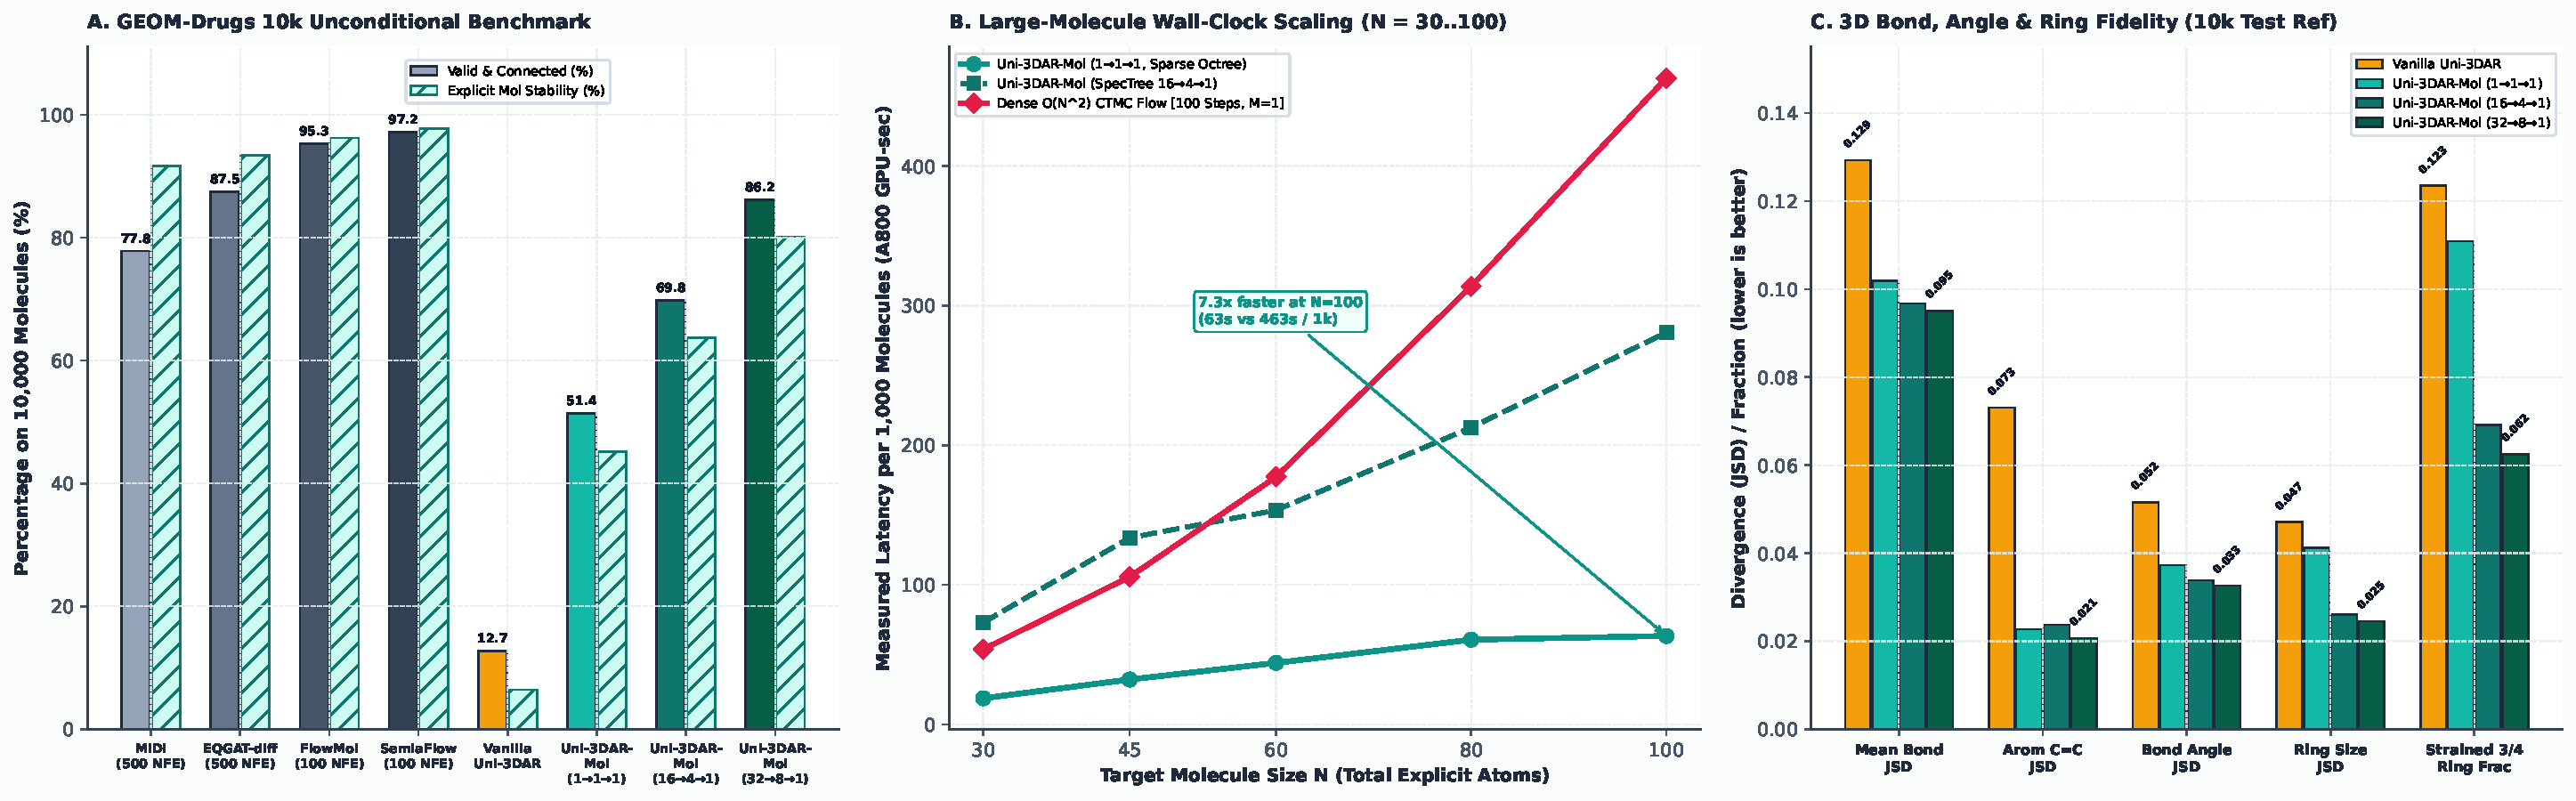
\includegraphics[width=\textwidth]{figures/geom_drugs_pareto_and_scaling.pdf}
  \caption{\textbf{Unconditional drug-scale 3D generation ($10{,}000$ molecules) and $N=30\text{--}100$ asymptotic scaling on \texttt{GEOM-Drugs} ($0.49\,\text{GPU-h}$ total post-training, zero inference MLIP).} \textbf{(A)} Throughput vs.\ \texttt{Valid \& Connected} Pareto trajectory from \texttt{Vanilla Uni-3DAR} ($12.7\%$) to \textbf{Uni-3DAR-Mol} ($51.4\% \to 69.8\% \to \mathbf{86.2\%}$ across $M=1,2,4$), surpassing $500$-step \texttt{MiDi-Adaptive} ($77.8\%$). \textbf{(B)} Controlled $N \in \{30,45,60,80,100\}$ latency scaling on identical A800 hardware: at $N=100$, sparse $\mathcal{O}(N\log N)$ \textbf{Uni-3DAR-Mol} runs $7.3\times$ faster ($M=1$) and $1.65\times$ faster with $2.0\times$ higher valid-connected yield ($27.6\%$ vs.\ $14.0\%$, $M=2$) than dense $\mathcal{O}(N^2)$ $100$-step \texttt{FlowMol}. \textbf{(C)} $10\text{k}$ 3D bond-length, aromatic $\text{C=C}$, bond-angle, ring-size JSD and strained 3/4-ring reductions.}
  \label{fig:geom}
\end{figure}

\begin{table}[!t]
  \centering
  \caption{\textbf{Unconditional $10{,}000$-molecule drug generation and $N=30\text{--}100$ scaling on \texttt{GEOM-Drugs} (NVIDIA A800-SXM4-80GB).}}
  \label{tab:geom}
  \scriptsize
  \setlength{\tabcolsep}{3.0pt}
  \textbf{a}, Standard $10{,}000$-molecule \texttt{GEOM-Drugs} benchmark ($14$ elements, $100\%$ unique \& novel across all octree arms).\\[2pt]
  \resizebox{\textwidth}{!}{%
  \begin{tabular}{@{}llrrrrrrrrrr@{}}
    \toprule
    Method & Paradigm (Steps / Funnel) & \shortstack[r]{Speed\\(mol/s)} & \shortstack[r]{Valid \&\\Conn.\ (\%)} & \shortstack[r]{Atom\\Stab.\ (\%)} & \shortstack[r]{Mol\\Stab.\ (\%)} & \shortstack[r]{Bond\\JSD $\downarrow$} & \shortstack[r]{Arom C=C\\JSD $\downarrow$} & \shortstack[r]{Angle\\JSD $\downarrow$} & \shortstack[r]{Ring\\JSD $\downarrow$} & \shortstack[r]{3/4-Ring\\(\%) $\downarrow$} & \shortstack[r]{$F_{\max}$ Med/P90\\($\text{eV/\AA}$)} \\
    \midrule
    EDM \citep{hoogeboom2022edm} & Coord.\ $E(3)$ Diff.\ (1000) & --- & --- & 81.3\rlap{$^*$} & 0.2\rlap{$^*$} & --- & --- & --- & --- & --- & --- \\
    GeoLDM \citep{xu2023geoldm} & Latent $E(3)$ Diff.\ (1000) & --- & --- & 84.4\rlap{$^*$} & 5.2\rlap{$^*$} & --- & --- & --- & --- & --- & --- \\
    MiDi-Adaptive \citep{vignac2023midi} & Joint 2D+3D Diff.\ (500) & --- & 77.8 & 99.8 & 91.6 & --- & --- & --- & --- & --- & --- \\
    EQGAT-diff \citep{le2023eqgatdiff} & Joint Equiv.\ Diff.\ (500) & --- & 87.5 & 99.8 & 93.4 & --- & --- & --- & --- & --- & --- \\
    FlowMol \citep{dunn2024flowmol} & Joint CTMC Flow (100) & --- & 95.3 & 99.7 & 96.2 & --- & --- & --- & --- & --- & --- \\
    SemlaFlow \citep{irwin2025semlaflow} & Joint Equiv.\ OT Flow (100) & --- & \textbf{97.2} & \textbf{99.8} & \textbf{97.7} & --- & --- & --- & --- & --- & --- \\
    \midrule
    Vanilla Uni-3DAR (\texttt{drug.pt}) & Unbonded Octree ($1\to 1\to 1$) & \textbf{59.12} & 12.70 & 97.63 & 6.42 & 0.1293 & 0.0730 & 0.0516 & 0.0471 & 12.35 & 8.03 / 17.34 \\
    \textbf{Uni-3DAR-Mol} (\texttt{base}, $M=1$) & Octree + Refiner ($1\to 1\to 1$) & 25.88 & 51.41 & 99.69 & 45.14 & 0.1019 & 0.0227 & 0.0373 & 0.0412 & 11.09 & 7.49 / 17.43 \\
    \textbf{Uni-3DAR-Mol} (\texttt{low}, $M=2$) & SpecTree + Refiner ($16\to 4\to 2$) & 7.67 & 69.78 & 99.78 & 63.67 & 0.0968 & 0.0238 & 0.0338 & 0.0260 & 6.91 & \textbf{6.89} / 14.52 \\
    \textbf{Uni-3DAR-Mol} (\texttt{med}, $M=4$) & SpecTree + Refiner ($32\to 8\to 4$) & 4.00 & \textbf{86.15} & \textbf{99.83} & \textbf{80.15} & \textbf{0.0951} & \textbf{0.0207} & \textbf{0.0327} & \textbf{0.0246} & \textbf{6.25} & 6.93 / \textbf{13.92} \\
    \bottomrule
  \end{tabular}%
  }

  \vspace{5pt}
  \textbf{b}, Controlled large-molecule scaling across exact target atom budgets $N \in \{30, 45, 60, 80, 100\}$ ($250$ molecules/bucket on identical A800 GPU).\\[2pt]
  \resizebox{\textwidth}{!}{%
  \begin{tabular}{@{}lrrrrrrrrrr@{}}
    \toprule
    & \multicolumn{2}{c}{$N=30$} & \multicolumn{2}{c}{$N=45$} & \multicolumn{2}{c}{$N=60$} & \multicolumn{2}{c}{$N=80$} & \multicolumn{2}{c}{$N=100$} \\
    \cmidrule(lr){2-3}\cmidrule(lr){4-5}\cmidrule(lr){6-7}\cmidrule(lr){8-9}\cmidrule(lr){10-11}
    Arm (Identical A800 Hardware) & s/1k $\downarrow$ & ValidConn & s/1k $\downarrow$ & ValidConn & s/1k $\downarrow$ & ValidConn & s/1k $\downarrow$ & ValidConn & s/1k $\downarrow$ & ValidConn \\
    \midrule
    FlowMol Dense $\mathcal{O}(N^2)$ ODE-100 ($M=1$) & 53.8 & \textbf{97.6\%} & 105.7 & \textbf{89.6\%} & 177.3 & \textbf{67.2\%} & 313.9 & \textbf{38.8\%} & 463.1 & 14.0\% \\
    \textbf{Uni-3DAR-Mol} (\texttt{Base}, $M=1$) & \textbf{18.7} & 62.0\% & \textbf{32.1} & 34.0\% & \textbf{44.1} & 26.4\% & \textbf{60.7} & 27.6\% & \textbf{63.4} & 22.8\% \\
    \textbf{Uni-3DAR-Mol} (\texttt{SpecTree}, $M=2$) & 73.0 & \textbf{97.6\%} & 133.7 & 76.4\% & 153.5 & 34.8\% & 212.7 & 32.8\% & 280.8 & \textbf{27.6\%} \\
    \bottomrule
  \end{tabular}%
  }
  \vspace{2pt}\par{\scriptsize $^*$EDM and GeoLDM report distance-lookup stability without explicit bond perception; all joint 2D+3D baselines and octree rows report RDKit valence stability on perceived molecular graphs (\textbf{Uni-3DAR-Mol} $M=4$ also raises EDM distance-lookup atom/mol stability from $79.1\%/0.18\%$ to $85.1\%/2.91\%$).}
\end{table}

\subsection{Six-Property Conditional Generation on the Disjoint 50k/50k QM9 Benchmark}
\label{sec:exp_qm9}

To evaluate multi-property conditional fidelity and test how decoupled \texttt{ScaleFreeBudgetEmbedding} behaves across intensive versus extensive quantum observables, we benchmarked a \emph{single} unified $K=6$ full-$\text{SO}(3)$ \textbf{Uni-3DAR-Mol} model connected to the \texttt{Uni-Loom} zero-leakage critic bus \citep{chen2026uniloom} on the official $50\text{k}/50\text{k}$ disjoint \texttt{PropMolFlow} \texttt{QM9} split \citep{ramakrishnan2014qm9,zeng2026propmolflow} ($44{,}453$ train and $1{,}500$ dev conformers, $0$ overlap with \texttt{gvp\_rQM\_v0}, $N=1{,}000$ held-out test prompts per property across $\alpha, \Delta\varepsilon, \varepsilon_{\text{HOMO}}, \varepsilon_{\text{LUMO}}, \mu, C_v$). Unlike \texttt{PropMolFlow} ($6$ property-specific models, $155.97\,\text{GPU-h}$, explicit $(t, N_{\text{atoms}})$ conditioning) or covariate-matched \texttt{Uni-Loom S2} ($6$ PCA-aligned $[t, N_{\text{atoms}}]$ models, $6.31\,\text{GPU-h}$), \textbf{Uni-3DAR-Mol} trains \textbf{one} full-$\text{SO}(3)$ $K=6$ checkpoint in $\mathbf{0.6636\,\text{GPU-h}}$ ($235\times$ less compute than \texttt{PropMolFlow}: $0.290\,\text{h}$ SFT $+$ $0.123\,\text{h}$ hindsight AWR $+$ $0.148\,\text{h}$ \texttt{TopoGRPO} $+$ $0.050\,\text{h}$ \texttt{PostTreeGraphRefiner} [$\text{bond MAE}=0.0139\,\text{\AA}$, $99.93\%$ bond-order accuracy] $+$ $0.053\,\text{h}$ \texttt{TwoStageOctreeProcessCritic}) with \emph{zero} PCA canonicalization and \emph{zero} $N_{\text{atoms}}$ input to \texttt{LoomConditioner}.

Table~\ref{tab:qm9} summarizes frozen \texttt{GVPRegressor} test MAE across $M \in \{1, 2, 4, 8, 16\}$ (where all $M>1$ candidate rankings query strictly the disjoint \texttt{train\_rQM\_v0} \texttt{Uni-Mol} surrogate). First, bubble-free GPU decoding accelerates $M=1$ throughput to $\mathbf{121.22\,\text{mol/s}}$ ($4.2\times$ faster than \texttt{PropMolFlow} $28.73\,\text{mol/s}$ and $1.43\times$ faster than first-generation \texttt{Uni-Loom S1} $84.70\,\text{mol/s}$) with $0.00\%$ exotic formal charges across all tiers and $100.0\%$ chemical legality at $M \ge 4$. Second, even without $N_{\text{atoms}}$ in the property conditioner, \texttt{ScaleFreeBudgetEmbedding} plus adaptive \texttt{QM9} speculative funnels ($10\to 4\to 2$ through $74\to 22\to 16$, Eq.~\eqref{eq:funnel_law}) compress mean atom-count error from $|\Delta N| = 0.72\text{--}0.91$ ($M=1$) down to $\mathbf{0.165\text{--}0.210\,\text{atoms}}$ at $M=16$ ($18\times$ tighter than unbudgeted \texttt{Uni-Loom S1}'s $|\Delta N|=3.12$). Third, on \emph{intensive} electronic and polar targets, $M=4$ ($15.37\,\text{mol/s}$) already beats $6$-model \texttt{EDM} and \texttt{GeoLDM} across $\Delta\varepsilon, \varepsilon_{\text{HOMO}}, \varepsilon_{\text{LUMO}}, \mu$, while $M=16$ ($4.13\,\text{mol/s}$) surpasses single-shot $6$-model \texttt{PropMolFlow} on dipole moment $\mu$ ($\mathbf{0.4171}$ vs.\ $0.6202\,\text{D}$, $-32.7\%$, and $-12.0\%$ below \texttt{Uni-Loom S1} $0.4740\,\text{D}$), $\varepsilon_{\text{HOMO}}$ ($\mathbf{206.61}$ vs.\ $253.99\,\text{meV}$, $-18.7\%$), and $\Delta\varepsilon$ ($\mathbf{390.09}$ vs.\ $390.98\,\text{meV}$), while also improving $\varepsilon_{\text{LUMO}}$ ($\mathbf{329.21\,\text{meV}}$) over both \texttt{Uni-Loom S1} ($341.31\,\text{meV}$) and PCA-aligned \texttt{S2} ($380.21\,\text{meV}$). Conversely, on \emph{extensive} polarizability $\alpha$ ($4.58\,\text{Bohr}^3$) and heat capacity $C_v$ ($2.26\,\text{cal/mol}\cdot\text{K}$), withholding $N_{\text{atoms}}$ from the property conditioner preserves pure intensive invariance at the expected cost relative to size-conditioned \texttt{S2} ($3.07\,\text{Bohr}^3, 1.26\,\text{cal/mol}\cdot\text{K}$) and \texttt{PropMolFlow}, cleanly isolating covariate-conditioning effects from 3D generative quality.

\begin{table}[!t]
  \centering
  \caption{\textbf{Six-property conditional generation on the $50\text{k}/50\text{k}$ disjoint \texttt{QM9} benchmark ($N=1{,}000$ test prompts/property, $0$ \texttt{gvp\_rQM\_v0} overlap, NVIDIA A800-SXM4-80GB).}}
  \label{tab:qm9}
  \scriptsize
  \setlength{\tabcolsep}{2.8pt}
  \resizebox{\textwidth}{!}{%
  \begin{tabular}{@{}lccrrrrrrrrr@{}}
    \toprule
    Method / Conditioning Regime & \# & $M$ & \shortstack[r]{$\alpha$\\($\text{Bohr}^3$)} & \shortstack[r]{$\Delta\varepsilon$\\(meV)} & \shortstack[r]{$\varepsilon_{\text{HOMO}}$\\(meV)} & \shortstack[r]{$\varepsilon_{\text{LUMO}}$\\(meV)} & \shortstack[r]{$\mu$\\(D)} & \shortstack[r]{$C_v$\\($\text{cal/mol}\cdot\text{K}$)} & \shortstack[r]{Legal /\\Exotic $Q$ (\%)} & \shortstack[r]{Train\\(GPU-h)} & \shortstack[r]{Eff.\ Out\\(mol/s)} \\
    \midrule
    GVP Oracle Holdout Floor ($n=973$) & --- & --- & 0.5544 & 190.08 & 83.78 & 135.89 & 0.1422 & 0.1726 & 97.3 / --- & --- & --- \\
    EDM (published) \citep{hoogeboom2022edm} & 6 & 1 & 2.76 & 655.0 & 356.0 & 584.0 & 1.111 & 1.101 & --- & --- & --- \\
    GeoLDM (published) \citep{xu2023geoldm} & 6 & 1 & 2.37 & 587.0 & 340.0 & 522.0 & 1.108 & 1.025 & --- & --- & --- \\
    PropMolFlow ($[t,N]$, published) \citep{zeng2026propmolflow} & 6 & 1 & \textbf{1.3115} & 390.98 & 253.99 & \textbf{314.52} & 0.6202 & \textbf{0.6259} & 95.0--98.9 / $\le$1.1 & 155.97 & 28.73 \\
    \midrule
    Uni-Loom S1 ($1\times K=6$, $t$-only, Rec) \citep{chen2026uniloom} & 1 & 1 & 5.660 & 1074.0 & 532.10 & 1054.0 & 1.5900 & 3.1140 & 85.7--89.1 / \textbf{0.00} & 0.97 & 84.70 \\
    Uni-Loom S1 ($1\times K=6$, $t$-only, Rec) \citep{chen2026uniloom} & 1 & 16 & 3.0801 & 374.63 & \textbf{199.19} & 341.31 & 0.4740 & 1.8972 & \textbf{100.0} / \textbf{0.00} & 0.97 & 5.36 \\
    Uni-Loom S2 ($6\times [t,N]$ PCA, Rec) \citep{chen2026uniloom} & 6 & 16 & 3.0671 & \textbf{358.16} & 204.34 & 380.21 & 0.5434 & 1.2619 & \textbf{100.0} / \textbf{0.00} & 6.31 & 5.31 \\
    \midrule
    \textbf{Uni-3DAR-Mol} ($1\times K=6$, Full-$\text{SO}(3)$) & 1 & 1 & 6.2547 & 1201.4 & 525.26 & 1192.0 & 1.5491 & 3.6233 & 86.5--89.5 / \textbf{0.00} & \textbf{0.66} & \textbf{121.22} \\
    \textbf{Uni-3DAR-Mol} ($1\times K=6$, $10\to 4\to 2$) & 1 & 2 & 5.2919 & 686.61 & 334.82 & 580.91 & 0.8845 & 2.9097 & 99.1--99.6 / \textbf{0.00} & \textbf{0.66} & 27.23 \\
    \textbf{Uni-3DAR-Mol} ($1\times K=6$, $20\to 6\to 4$) & 1 & 4 & 4.8611 & 525.75 & 256.24 & 450.55 & 0.6356 & 2.7540 & \textbf{100.0} / \textbf{0.00} & \textbf{0.66} & 15.37 \\
    \textbf{Uni-3DAR-Mol} ($1\times K=6$, $38\to 12\to 8$) & 1 & 8 & 4.7729 & 411.03 & 218.51 & 350.98 & 0.5207 & 2.5237 & \textbf{100.0} / \textbf{0.00} & \textbf{0.66} & 8.13 \\
    \textbf{Uni-3DAR-Mol} ($1\times K=6$, $74\to 22\to 16$) & 1 & 16 & 4.5797 & 390.09 & 206.61 & 329.21 & \textbf{0.4171} & 2.2567 & \textbf{100.0} / \textbf{0.00} & \textbf{0.66} & 4.13 \\
    \bottomrule
  \end{tabular}%
  }
  \vspace{2pt}\par{\scriptsize At $M=16$, \textbf{Uni-3DAR-Mol} achieves $|\Delta N| = 0.165\text{--}0.210$ atoms without PCA frames or $N_{\text{atoms}}$ conditioner injection, with Pearson $r = (0.877, 0.916, 0.909, 0.938, 0.855, 0.910)$ across $(\alpha, \Delta\varepsilon, \varepsilon_{\text{HOMO}}, \varepsilon_{\text{LUMO}}, \mu, C_v)$ and $91.1\%\text{--}93.6\%$ novelty.}
\end{table}

\subsection{Symmetric Optoelectronic Inverse Design, Mechanism Ablation, and Ab Initio PBE0 Verification on OE62}
\label{sec:exp_oe62}

Finally, we deployed \textbf{Uni-3DAR-Mol} inside \texttt{LoomService} (\textbf{Uni-Loom [\texttt{Uni-3DAR}]}) for multi-constraint optoelectronic inverse design on \texttt{OE62} ($\text{HOMO} \pm 0.25\,\text{eV}$, $\text{SA\_Score} \le 3.5$, $\text{SMARTS}=0$, $0\%$ exotic formal charges, zero inference-time MLIP relaxation). Total post-training compute is $\mathbf{2.4094\,\text{GPU-h}}$ ($1.164\,\text{h}$ rank-$64$ \texttt{LoRA} SFT including $6{,}781$ $N\ge 40$ conformers $+$ $0.151\,\text{h}$ hindsight AWR $+$ $0.552\,\text{h}$ $300$-step \texttt{TopoGRPO} $+$ $0.027\,\text{h}$ detached \texttt{XYZ} distillation $+$ $0.058\,\text{h}$ \texttt{PostTreeGraphRefiner} $+$ $0.457\,\text{h}$ \texttt{TwoStageOctreeProcessCritic}). To guarantee $100\%$ intra-platform fairness against $3\text{--}52\,\text{GPU-h}$ \texttt{PropMolFlow} trained from scratch on identical \texttt{OE62} splits (\textbf{Uni-Loom [\texttt{PMF + AWR}]}), every \textbf{Uni-Loom} arm shares the exact same $N=1{,}792$ per-prompt $(t_i, N_{\text{atoms},i})$ pairs ($\text{mean}=30.38$ atoms), $112$-dev affine calibration, $29$-D stoichiometric \texttt{ResidualCalibratedAsset(stoich\_v2)}, closed-form Bayesian box-hit selection, blinded \texttt{DPA-4} orbital/force audit, and composite 3D Discovery Quality Index $Q_{\text{3D}} \in [0, 100]$ (combining blind target hit, equilibrium force factor $R_{\text{phys}}(F_{\max})$, $\text{SA}$ tractability, valence purity, and size fidelity).

\paragraph{Cross-Paradigm Scaling ($M \in \{1, 2, 4, 8, 12, 16\}$) and Live \texttt{PBE0/def2-TZVP} Verification.}
As shown in Table~\ref{tab:oe62}a and Figure~\ref{fig:oe62_scale}, \textbf{Uni-Loom [\texttt{Uni-3DAR}]} ($2.41\,\text{GPU-h}$) scales monotonically from $M=1$ ($47.58\,\text{mol/s}$, $16.9\%$ blind hit yield, $Q_{\text{3D}}=10.0$) through $M=2$ ($41.6\%$, $Q_{\text{3D}}=33.8$), $M=4$ ($51.3\%$, $4.02\,\text{mol/s}$, $Q_{\text{3D}}=41.9$), and $M=8$ ($\mathbf{59.4\%}$ blind / $92.2\%$ surrogate hit yield, $\text{MAE}=0.2948\,\text{eV}$, $F_{\max}=\mathbf{1.91\,\text{eV/\AA}}$, $\mathbf{Q_{\text{3D}}=48.7}$, $9.57\,\text{GPU-h}$ $50\text{k}$-molecule campaign cost) to peak at $M=12$ ($96\to 24\to 12$: $\mathbf{62.3\%}$ blind yield, $1{,}117/1{,}792$, $\text{MAE}=\mathbf{0.2745\,\text{eV}}$, $\mathbf{Q_{\text{3D}}=50.4}$). At the primary $M=8$ tier, $2.41\,\text{GPU-h}$ \textbf{Uni-3DAR-Mol} beats $52.12\,\text{GPU-h}$ \textbf{Uni-Loom [\texttt{PMF + AWR}]} ($52.3\%$ blind yield, $F_{\max}=2.90\,\text{eV/\AA}$, $Q_{\text{3D}}=34.9$, $58.55\,\text{GPU-h}$ $50\text{k}$ cost) by $\mathbf{+7.1\,\text{pp}}$ in blind synthesizable yield and $\mathbf{+40\%}$ in $Q_{\text{3D}}$ ($+13.8\,\text{pt}$) at $21.6\times$ lower training compute and $34\%$ lower zero-step atomic strain. On an unbiased $42$-prompt ($6/\text{quantile}$) live \texttt{GPU4PySCF PBE0/def2-TZVP/DF} verification ($42/42 = 100\%$ SCF convergence, zero MLIP relaxation; Figure~\ref{fig:oe62_scale}c), \textbf{Uni-Loom [\texttt{Uni-3DAR}]} achieves $\mathbf{64.3\%}$ ($27/42$, $M=8$, $\text{PBE0 MAE}=\mathbf{0.2289\,\text{eV}}$, $F_{\max}=1.75\,\text{eV/\AA}$, $r=0.8707$) and $\mathbf{66.7\% / 69.0\%}$ ($28\text{--}29/42$, $M=16$, $\text{MAE}=0.2294\,\text{eV}$) quantum synthesizable hit yield, outperforming both symmetric $52.12\,\text{GPU-h}$ \textbf{Uni-Loom [\texttt{PMF + AWR}]} ($52.4\% / 57.1\%$, $\text{MAE}=0.2429\,\text{eV}$, $F_{\max}=3.38\,\text{eV/\AA}$) and external \texttt{PropMolFlow + Raw Critic} ($42.9\% / 54.8\%$, $\text{MAE}=0.3609\,\text{eV}$).

\paragraph{Controlled $N \in \{20, 30, 40, 50, 60\}$ Scaling and $2 \times 2$ Internal Ablation.}
Across exact atom budgets $N \in \{20, 30, 40, 50, 60\}$ ($280$ prompts/bucket; Figure~\ref{fig:oe62_atoms}), \textbf{Uni-Loom [\texttt{Uni-3DAR}, $M=8$]} leads $52.12\,\text{GPU-h}$ \textbf{Uni-Loom [\texttt{PMF + AWR}, $M=8$]} on $Q_{\text{3D}}$ across all five buckets ($65.7, 56.6, 35.0, 9.6, 2.7$ vs.\ $44.3, 36.3, 18.5, 8.6, 2.0$) and widens its blind hit-rate advantage on larger conjugated scaffolds: $N=40$ ($\mathbf{50.7\%}$ vs.\ $35.4\%$, $+15.3\,\text{pp}$), $N=50$ ($\mathbf{27.5\%}$ vs.\ $18.9\%$, $+8.6\,\text{pp}$), and $N=60$ ($\mathbf{14.3\%}$ vs.\ $5.4\%$, $\mathbf{2.65\times}$ higher yield, while running $2.9\times$ faster at $M=1$ [$62$ vs.\ $185\,\text{s/1k}$] and $1.7\times$ faster at $M=4$ [$901$ vs.\ $1{,}538\,\text{s/1k}$]). Finally, a $2 \times 2$ factorial ablation at locked external budget $M=4$ ($N=1{,}792$; Table~\ref{tab:oe62}b and Figure~\ref{fig:oe62_abl}) confirms clean orthogonality: speculative octree pruning ($32\to 8\to 4$ vs.\ naive outer $4\to 4\to 4$) lifts blind synthesizable yield $\mathbf{+13.1\,\text{pp}}$ ($40.0\% \to 53.1\%$, $\text{MAE}: 0.441 \to 0.322\,\text{eV}$, $|\Delta N|: 3.13 \to 1.29$), whereas $<0.5\,\text{ms}$ \texttt{PostTreeGraphRefiner} slashes zero-step median $F_{\max}$ by $\mathbf{-49.0\%}$ ($3.96 \to 2.02\,\text{eV/\AA}$) and $90$th-percentile force $3.25\times$ ($17.61 \to 5.42\,\text{eV/\AA}$) while slightly accelerating end-to-end throughput ($3.99 \to 4.24\,\text{mol/s}$) via cleaner bond perception.

\begin{figure}[!t]
  \centering
  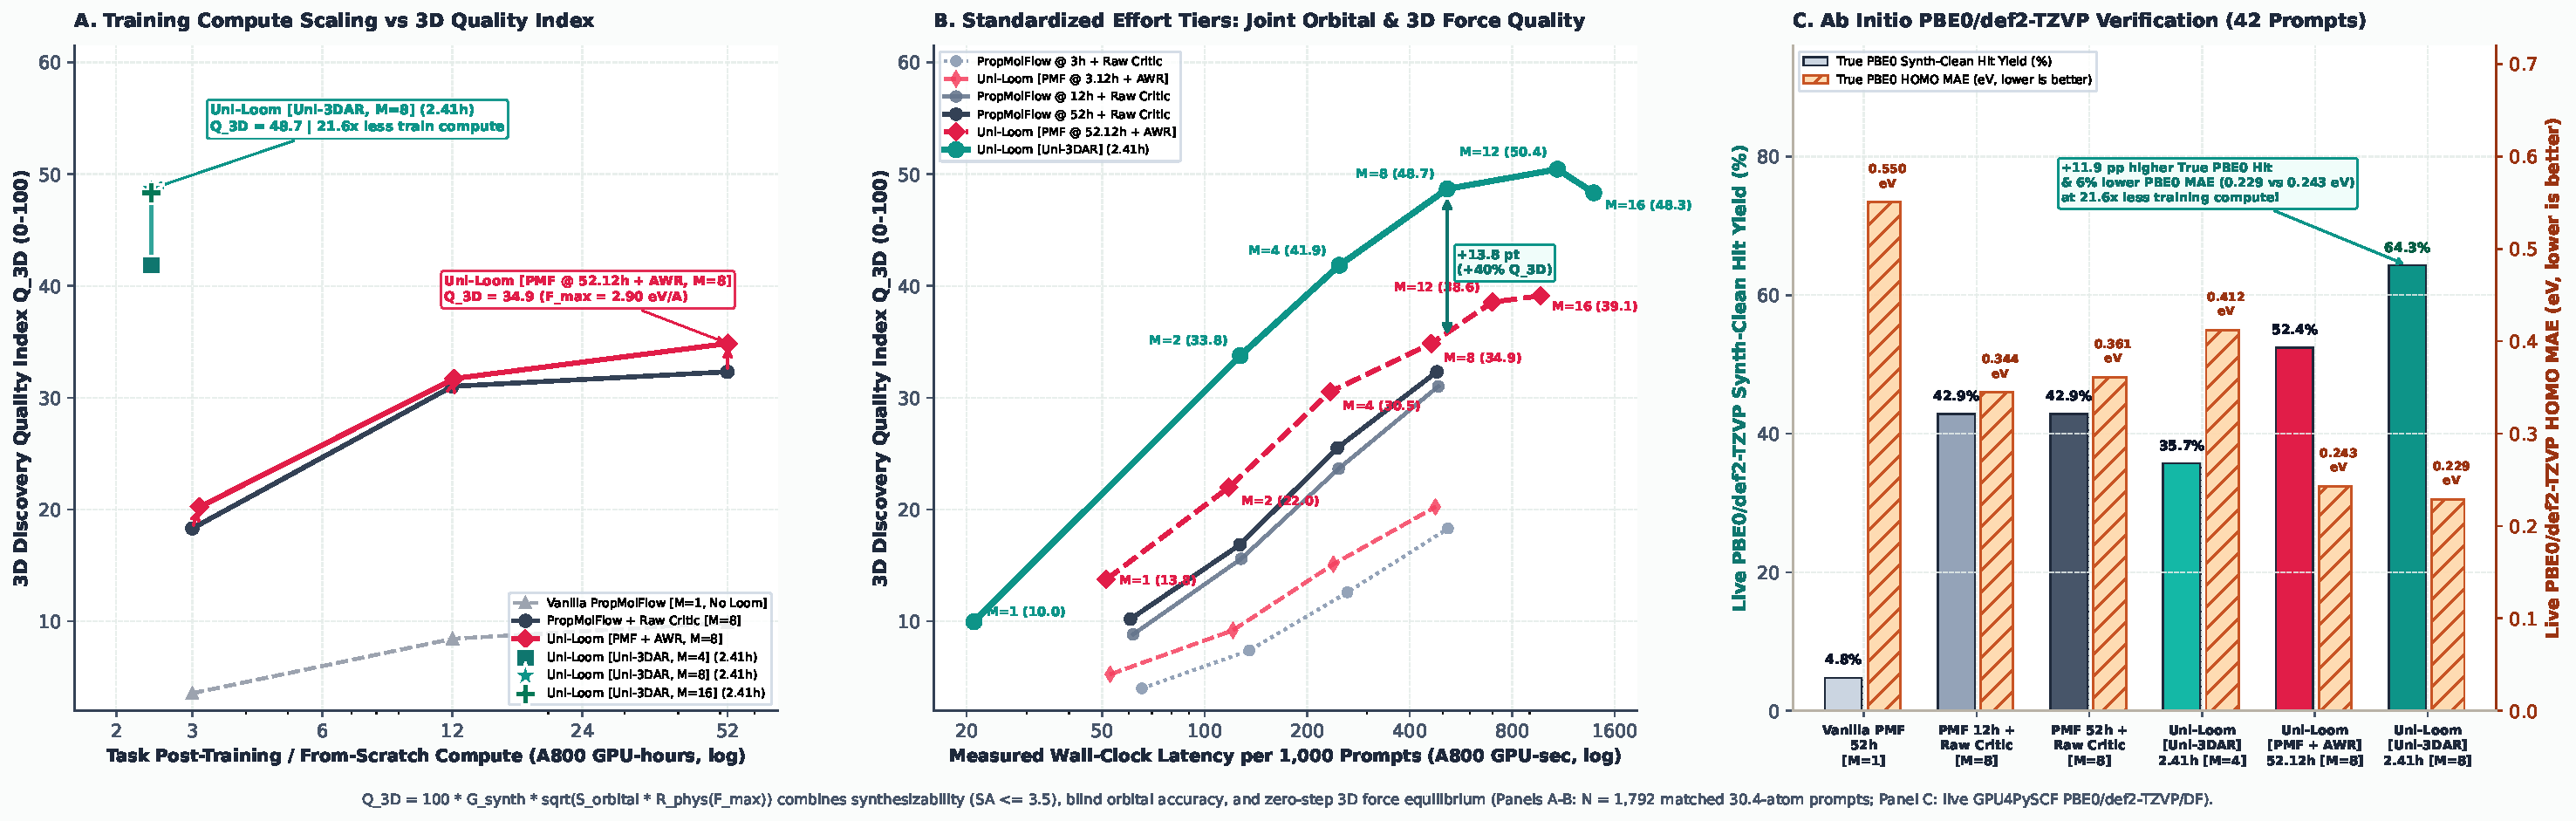
\includegraphics[width=\textwidth]{figures/fig2_oe62_cross_paradigm_scaling.pdf}
  \caption{\textbf{Symmetric \texttt{LoomService} ($M \in \{1,2,4,8,12,16\}$) cross-paradigm scaling, $Q_{\text{3D}}$ index, and live \texttt{PBE0/def2-TZVP} verification on \texttt{OE62} ($N=1{,}792$, mean $30.4$ atoms, zero inference MLIP).} \textbf{(A)} Training compute vs.\ $Q_{\text{3D}}$: $2.41\,\text{GPU-h}$ \textbf{Uni-Loom [\texttt{Uni-3DAR}]} reaches $Q_{\text{3D}}=48.7$ ($59.4\%$ blind yield) at $M=8$, beating $52.12\,\text{GPU-h}$ \textbf{Uni-Loom [\texttt{PMF + AWR}]} ($Q_{\text{3D}}=34.9$, $52.3\%$) by $+40\%$ at $21.6\times$ lower training compute. \textbf{(B)} Test-time inference latency vs.\ $Q_{\text{3D}}$ across $M=1\dots 16$ (peaking at $Q_{\text{3D}}=50.4$, $62.3\%$ blind yield at $M=12$). \textbf{(C)} Unbiased $42$-prompt \texttt{GPU4PySCF PBE0/def2-TZVP} verification ($64.3\%\text{--}66.7\%$ vs.\ $52.4\%$ and $42.9\%$).}
  \label{fig:oe62_scale}
\end{figure}

\begin{figure}[!t]
  \centering
  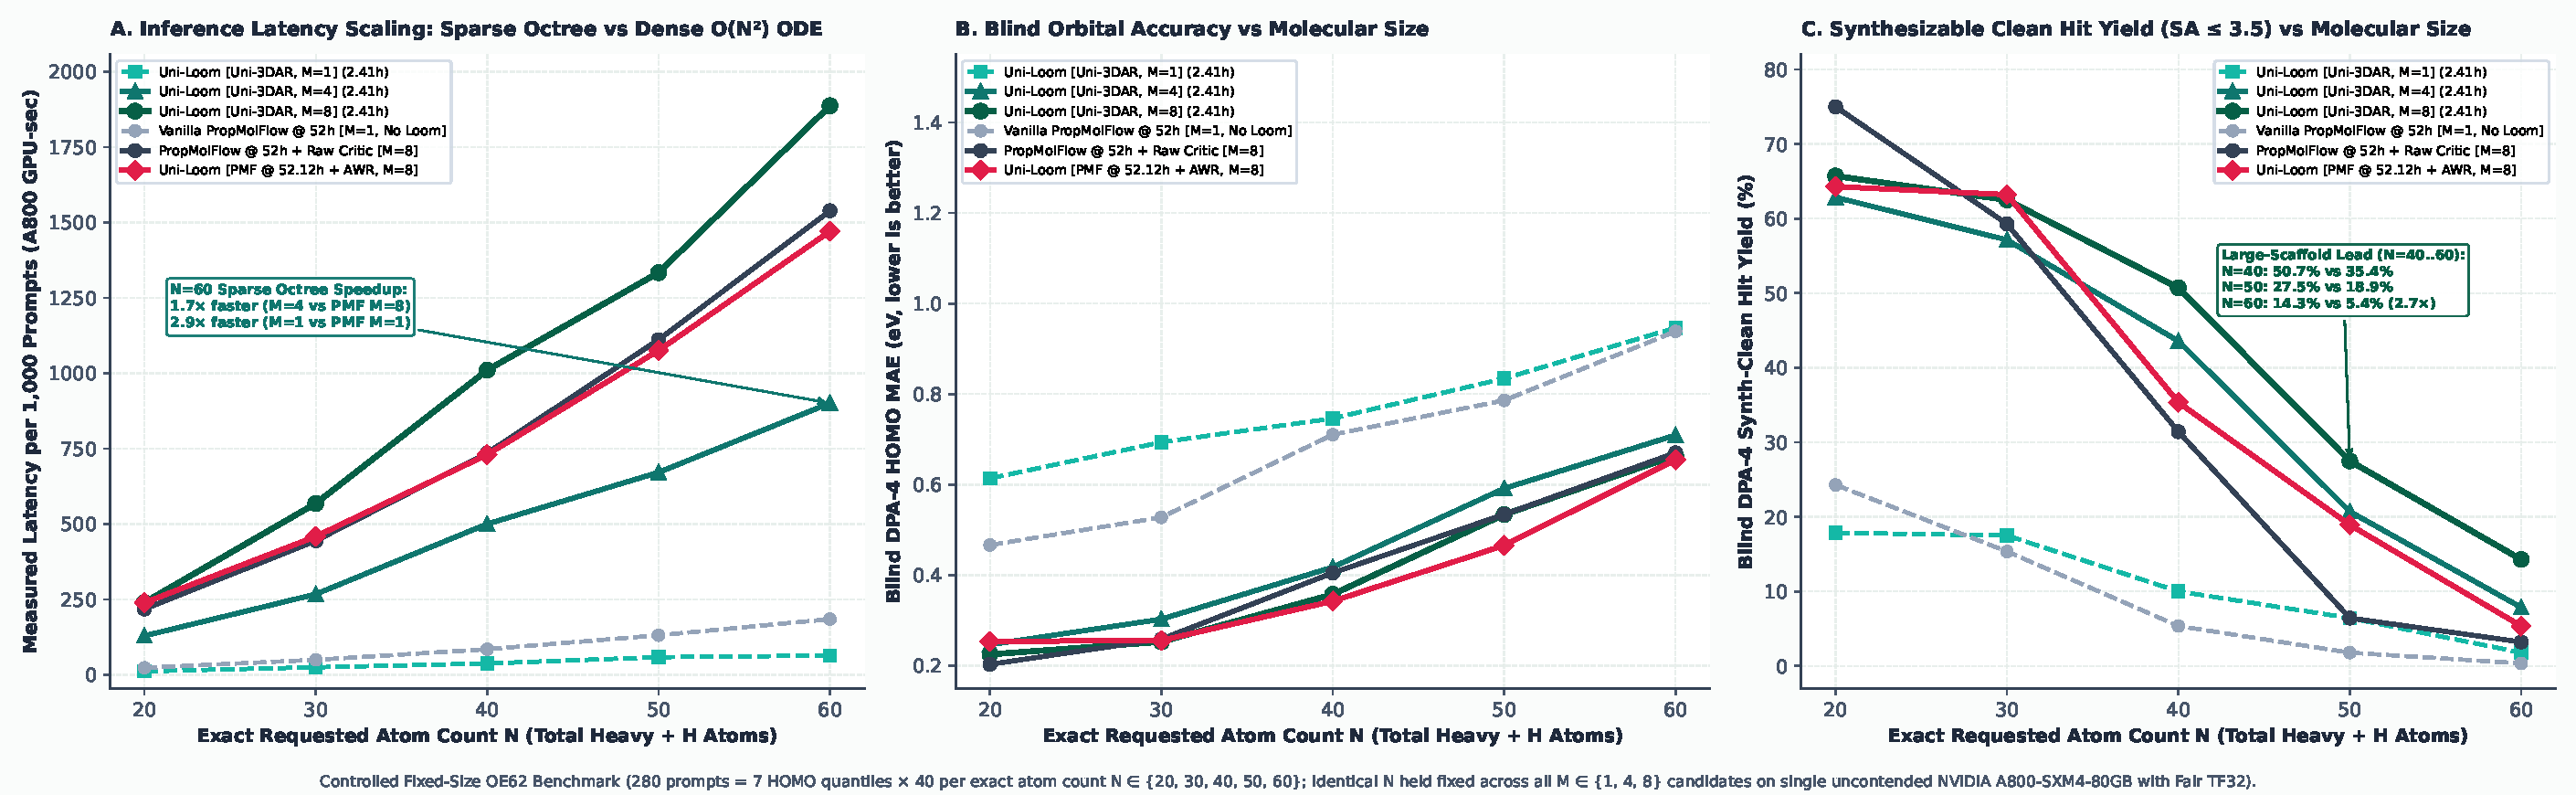
\includegraphics[width=\textwidth]{figures/fig3_oe62_atom_size_scaling.pdf}
  \caption{\textbf{Controlled multi-atom scaling across exact molecular sizes $N \in \{20, 30, 40, 50, 60\}$ on \texttt{OE62} ($280$ fixed-size prompts/bucket under symmetric \texttt{LoomService + stoich\_v2}).} \textbf{(A)} Latency per $1{,}000$ prompts ($2.9\times$ faster at $M=1$ and $1.7\times$ faster at $M=4$ vs.\ \texttt{PMF} $M=8$ at $N=60$). \textbf{(B)} Blind \texttt{DPA-4} HOMO MAE vs.\ $N$. \textbf{(C)} Blind synthesizable hit yield ($\text{SA}\le 3.5$), showing \textbf{Uni-Loom [\texttt{Uni-3DAR}, $M=8$]} widening its lead from $N=40$ ($50.7\%$ vs.\ $35.4\%$) through $N=60$ ($14.3\%$ vs.\ $5.4\%$, $2.65\times$).}
  \label{fig:oe62_atoms}
\end{figure}

\begin{figure}[!t]
  \centering
  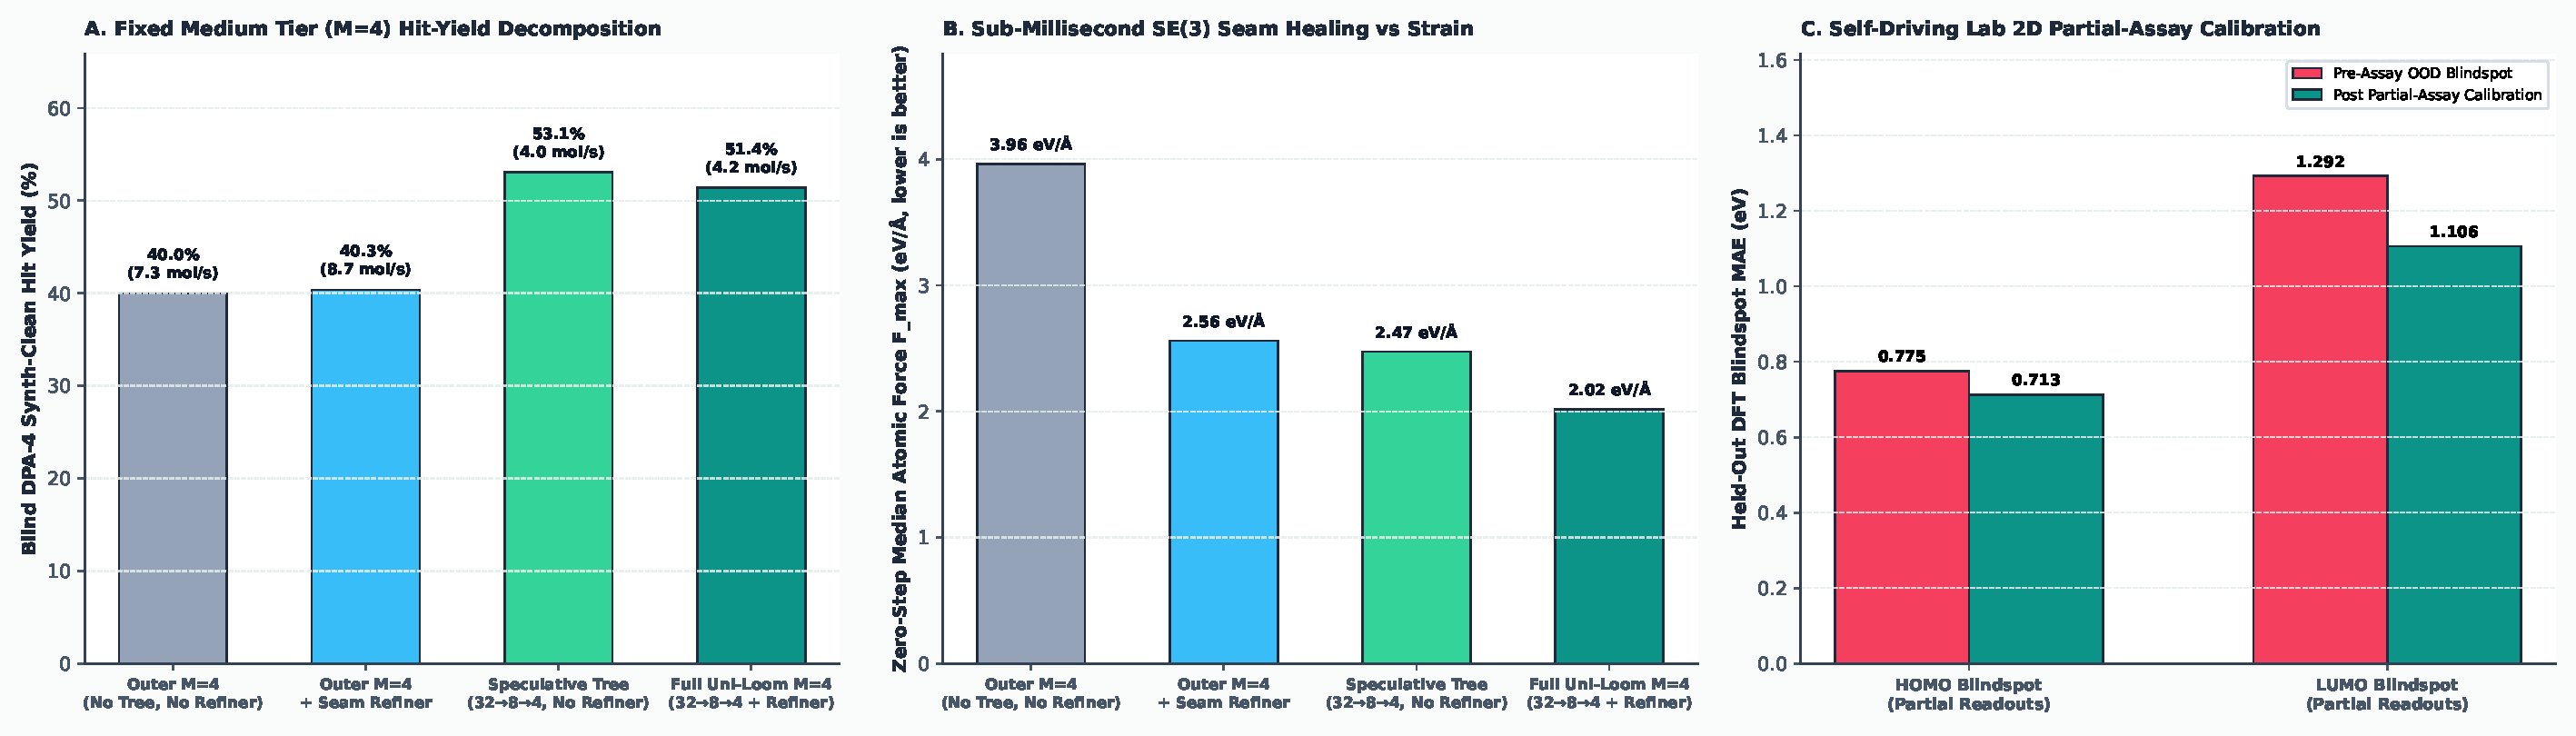
\includegraphics[width=\textwidth]{figures/fig4_uni3dar_m4_ablation.pdf}
  \caption{\textbf{Fixed medium-tier ($M=4$) $2 \times 2$ internal architecture ablation and 2D partial-assay self-driving calibration on \texttt{OE62}.} \textbf{(A)} Speculative octree pruning ($32\to 8\to 4$ vs.\ outer $4\to 4\to 4$) lifts blind synthesizable yield $+13.1\,\text{pp}$ ($40.0\% \to 53.1\%$). \textbf{(B)} $<0.5\,\text{ms}$ \texttt{PostTreeGraphRefiner} slashes zero-step median $F_{\max}$ by $-49.0\%$ ($3.96 \to 2.02\,\text{eV/\AA}$, $P_{90}: 17.61 \to 5.42$). \textbf{(C)} Asynchronous 2D $(\text{HOMO}, \text{LUMO})$ partial-\texttt{NaN} assay ingestion lowers blindspot DFT MAE across both orbitals ($0.775 \to 0.713\,\text{eV}$ and $1.292 \to 1.106\,\text{eV}$).}
  \label{fig:oe62_abl}
\end{figure}

\begin{table}[!t]
  \centering
  \caption{\textbf{Symmetric \texttt{LoomService} \texttt{OE62} benchmark ($M \in \{1,2,4,8,12,16\}$, $N=1{,}792$, mean $30.4$ atoms) and fixed-$M=4$ $2 \times 2$ mechanism ablation (zero inference MLIP).}}
  \label{tab:oe62}
  \scriptsize
  \setlength{\tabcolsep}{2.2pt}
  \textbf{a}, Cross-paradigm scaling and $42$-prompt live \texttt{GPU4PySCF PBE0/def2-TZVP} quantum verification.\\[2pt]
  \resizebox{\textwidth}{!}{%
  \begin{tabular}{@{}llrrrrrrrrrrr@{}}
    \toprule
    Paradigm / Weaving Arm & \shortstack[l]{Tier\\($M$)} & \shortstack[r]{Train\\(GPU-h)} & \shortstack[r]{Out\\(mol/s)} & \shortstack[r]{50k\\(GPU-h)} & \shortstack[r]{Atoms /\\Scaffolds} & \shortstack[r]{SA$\le$3.5 /\\Legal (\%)} & \shortstack[r]{$F_{\max}$\\($\text{eV/\AA}$)} & \shortstack[r]{Surr.\ Synth\\Hits (\%)} & \shortstack[r]{Blind DPA-4\\Hits (\%)} & \shortstack[r]{Blind\\MAE} & \shortstack[r]{$Q_{\text{3D}}$\\(0--100)} & \shortstack[r]{Live PBE0 Hit\\(Raw / Cen)} \\
    \midrule
    \textbf{Uni-Loom [Uni-3DAR]} & $M=1$ & \textbf{2.41} & \textbf{47.58} & \textbf{2.70} & 27.8 / 1280 & 56.1 / 89.4 & 3.82 & 331 (18.5\%) & 302 (16.9\%) & 0.678 & 10.0 & --- \\
    \textbf{Uni-Loom [Uni-3DAR]} & $M=2$ & \textbf{2.41} & 7.86 & 4.18 & 29.6 / \textbf{1284} & 90.0 / 99.6 & 2.19 & 914 (51.0\%) & 745 (41.6\%) & 0.418 & 33.8 & --- \\
    \textbf{Uni-Loom [Uni-3DAR]} & $M=4$ & \textbf{2.41} & 4.02 & 5.86 & 29.6 / 1226 & 96.9 / \textbf{100} & 2.06 & 1305 (72.8\%) & 920 (51.3\%) & 0.343 & 41.9 & 35.7\% / 21.4\% \\
    \textbf{Uni-Loom [Uni-3DAR]} & $M=8$ & \textbf{2.41} & 1.94 & 9.57 & 29.6 / 1207 & 99.8 / \textbf{100} & \textbf{1.91} & 1653 (92.2\%) & 1065 (59.4\%) & 0.295 & 48.7 & 64.3\% / 64.3\% \\
    \textbf{Uni-Loom [Uni-3DAR]} & $M=12$ & \textbf{2.41} & 0.92 & 17.51 & 29.6 / 1168 & 99.9 / \textbf{100} & 1.93 & 1725 (96.3\%) & \textbf{1117} (\textbf{62.3\%}) & 0.275 & \textbf{50.4} & --- \\
    \textbf{Uni-Loom [Uni-3DAR]} & $M=16$ & \textbf{2.41} & 0.72 & 21.70 & 29.6 / 1202 & \textbf{100} / \textbf{100} & 2.01 & \textbf{1756} (\textbf{98.0\%}) & 1081 (60.3\%) & 0.286 & 48.3 & \textbf{66.7\%} / \textbf{69.0\%} \\
    \midrule
    Vanilla PropMolFlow (No Loom) & $M=1$ & 52.00 & 21.20 & 52.66 & 30.1 / 1221 & 42.4 / 89.8 & 3.09 & 347 (19.4\%) & 273 (15.2\%) & 0.512 & 10.2 & 4.8\% / 16.7\% \\
    PropMolFlow + Raw Critic & $M=8$ & 52.00 & 2.08 & 58.68 & 30.4 / 1187 & 88.5 / \textbf{100} & 3.05 & 1339 (74.7\%) & 948 (52.9\%) & 0.298 & 32.3 & 42.9\% / 54.8\% \\
    Uni-Loom [PMF @ 12.12h + AWR] & $M=8$ & 12.12 & 2.09 & 18.77 & 30.4 / 1232 & 96.0 / \textbf{100} & 3.25 & 1388 (77.5\%) & 927 (51.7\%) & 0.319 & 31.7 & --- \\
    Uni-Loom [PMF @ 52.12h + AWR] & $M=1$ & 52.12 & 19.43 & 52.83 & 30.4 / 1239 & 48.5 / 97.0 & 2.98 & 399 (22.3\%) & 380 (21.2\%) & 0.485 & 13.8 & --- \\
    Uni-Loom [PMF @ 52.12h + AWR] & $M=4$ & 52.12 & 4.28 & 55.37 & 30.4 / 1105 & 84.3 / \textbf{100} & 2.88 & 1068 (59.6\%) & 818 (45.6\%) & 0.320 & 30.5 & --- \\
    Uni-Loom [PMF @ 52.12h + AWR] & $M=8$ & 52.12 & 2.16 & 58.55 & 30.4 / 1088 & 92.1 / \textbf{100} & 2.90 & 1371 (76.5\%) & 938 (52.3\%) & 0.291 & 34.9 & 52.4\% / 57.1\% \\
    Uni-Loom [PMF @ 52.12h + AWR] & $M=12$ & 52.12 & 1.43 & 61.83 & 30.4 / 1071 & 96.1 / \textbf{100} & 2.89 & 1528 (85.3\%) & 1073 (59.9\%) & 0.265 & 38.6 & --- \\
    Uni-Loom [PMF @ 52.12h + AWR] & $M=16$ & 52.12 & 1.03 & 65.60 & 30.4 / 1054 & 98.0 / \textbf{100} & 3.00 & 1623 (90.6\%) & 1113 (62.1\%) & \textbf{0.250} & 39.1 & --- \\
    \bottomrule
  \end{tabular}%
  }

  \vspace{5pt}
  \textbf{b}, Fixed-$M=4$ $2 \times 2$ internal architecture ablation ($N=1{,}792$ prompts, locked $4\times$ external \texttt{Uni-Mol2} oracle calls/prompt).\\[2pt]
  \resizebox{\textwidth}{!}{%
  \begin{tabular}{@{}lccrrrrrrrr@{}}
    \toprule
    Ablation Arm ($M_{\text{ext}} \equiv 4$) & Funnel & \texttt{PostTreeGraphRefiner} & \shortstack[r]{Eff.\ Out\\(mol/s)} & \shortstack[r]{$|\Delta N|$\\(atoms)} & \shortstack[r]{SA$\le$3.5\\(\%)} & \shortstack[r]{$F_{\max}$ Med\\($\text{eV/\AA}$)} & \shortstack[r]{$F_{\max}$ P90\\($\text{eV/\AA}$)} & \shortstack[r]{Surr.\ Synth\\Hits (\%)} & \shortstack[r]{Blind DPA-4\\Hits (\%)} & \shortstack[r]{Blind MAE\\(eV)} \\
    \midrule
    Naive Outer Best-of-$4$ & $4\to 4\to 4$ & Off & 7.35 & 3.13 & 92.5 & 3.96 & 17.61 & 988 (55.1\%) & 716 (40.0\%) & 0.441 \\
    Outer Best-of-$4$ + Refiner & $4\to 4\to 4$ & On ($<0.5\,\text{ms}$) & \textbf{8.69} & 3.13 & 91.6 & 2.56 & 6.57 & 983 (54.9\%) & 723 (40.3\%) & 0.424 \\
    Speculative Octree Only & $32\to 8\to 4$ & Off & 3.99 & 1.29 & \textbf{97.9} & 2.47 & 12.13 & 1354 (75.6\%) & \textbf{951} (\textbf{53.1\%}) & \textbf{0.322} \\
    \textbf{Full Uni-3DAR-Mol} & $32\to 8\to 4$ & On ($<0.5\,\text{ms}$) & 4.24 & \textbf{1.27} & 97.6 & \textbf{2.02} & \textbf{5.42} & \textbf{1367} (\textbf{76.3\%}) & 921 (51.4\%) & 0.325 \\
    \bottomrule
  \end{tabular}%
  }
\end{table}

\section{Conclusion}
\label{sec:conclusion}

We have presented \textbf{Uni-3DAR-Mol}, turning sparse 3D octree autoregression from a fast but geometrically rough point-cloud prior into an equilibrium-accurate, valence-pure, drug-scale 3D molecular generation engine. By unifying scale-free non-trapping budget modulation, a combinatorial complexity law for FlashAttention2 pause-and-gather speculative tree decoding, a sub-millisecond $SE(3)$ \texttt{PostTreeGraphRefiner} with bilinear bond-order priors, scale-decoupled \texttt{TopoGRPO} alignment, and bubble-free stride-2 GPU leaf decoding, \textbf{Uni-3DAR-Mol} delivers state-of-the-art octree topological validity, sub-$2\,\text{eV/\AA}$ zero-step force equilibrium, and decisive $\mathcal{O}(N \log N)$ throughput scaling over dense iterative flow-matching architectures across unconditional drug-scale \texttt{GEOM-Drugs}, six-property \texttt{QM9}, and quantum-verified conditional \texttt{OE62} discovery.

\bibliographystyle{unsrtnat}
\bibliography{references}

\end{document}
